\documentclass[12pt]{article}

%%%%%%%%%%%%%%%%%%%%%%%%%%%%%%%%%%%%%%%%%%%%%%%%%%%%%%%%%%%%%%%%%%%%%%%%
%% Customizações do abnTeX2 (http://abnTeX2.googlecode.com)           %%
%% para a Universidade Estadual do Ceara - UECE                       %%
%%                                                                    %%
%% This work may be distributed and/or modified under the             %%
%% conditions of the LaTeX Project Public License, either version 1.3 %%
%% of this license or (at your option) any later version.             %%
%% The latest version of this license is in                           %%
%%   http://www.latex-project.org/lppl.txt                            %%
%% and version 1.3 or later is part of all distributions of LaTeX     %%
%% version 2005/12/01 or later.                                       %%
%%                                                                    %%
%% This work has the LPPL maintenance status `maintained'.            %%
%%                                                                    %%
%% The Current Maintainer of this work is Thiago Nascimento           %%
%%                                                                    %%
%% Project available on: https://github.com/thiagodnf/uecetex2        %%
%%                                                                    %%
%% Further information about abnTeX2                                  %%
%% are available on http://abntex2.googlecode.com/                    %%
%%                                                                    %%
%%%%%%%%%%%%%%%%%%%%%%%%%%%%%%%%%%%%%%%%%%%%%%%%%%%%%%%%%%%%%%%%%%%%%%%%

% \documentclass[
%     a4paper,          % Tamanho da folha A4
%     12pt,             % Tamanho da fonte 12pt
%     chapter=TITLE,    % Todos os capitulos devem ter caixa alta
%     section=TITLE,    % Todas as secoes devem ter caixa alta
%     oneside,          % Usada para impressao em apenas uma face do papel
%     english,          % Hifenizacoes em ingles
%     spanish,          % Hifenizacoes em espanhol
%     brazil            % Ultimo idioma eh o idioma padrao do documento
% ]{abntex2}



% Importações de pacotes
\usepackage[utf8]{inputenc}                         % Acentuação direta
\usepackage[T1]{fontenc}                            % Codificação da fonte em 8 bits
\usepackage{graphicx}                               % Inserir figuras
\usepackage{amsfonts, amssymb, amsmath}             % Fonte e símbolos matemáticos
\usepackage{booktabs}                               % Comandos para tabelas
\usepackage{verbatim}                               % Texto é interpretado como escrito no documento
\usepackage{multirow, array}                        % Múltiplas linhas e colunas em tabelas
\usepackage{indentfirst}                            % Endenta o primeiro parágrafo de cada seção.
\usepackage{listings}                               % Utilizar codigo fonte no documento
\usepackage{xcolor}
\usepackage{microtype}                              % Para melhorias de justificação?
\usepackage[portuguese,ruled,lined]{algorithm2e}    % Escrever algoritmos
\usepackage{algorithmic}                            % Criar Algoritmos
\usepackage{float}                                  % Utilizado para criação de floats
\usepackage{amsgen}
\usepackage{lipsum}                                 % Usar a simulação de texto Lorem Ipsum
%\usepackage{titlesec}                               % Permite alterar os títulos do documento
\usepackage{tocloft}                                % Permite alterar a formatação do Sumário
\usepackage{etoolbox}                               % Usado para alterar a fonte da Section no Sumário
\usepackage[nogroupskip,nonumberlist,acronym]{glossaries}                % Permite fazer o glossario
\usepackage{caption}                                % Altera o comportamento da tag caption
\usepackage[num, abnt-emphasize=bf, bibjustif, recuo=0cm, abnt-etal-cite=2, abnt-etal-list=0]{abntex2cite}  % Citações padrão ABNT
%\usepackage[bottom]{footmisc}                      % Mantém as notas de rodapé sempre na mesma posição
%\usepackage{times}                                 % Usa a fonte Times
\usepackage{mathptmx}                               % Usa a fonte Times New Roman
%\usepackage{lmodern}                               % Usa a fonte Latin Modern
%\usepackage{subfig}                                % Posicionamento de figuras
%\usepackage{scalefnt}                              % Permite redimensionar tamanho da fonte
%\usepackage{color, colortbl}                        % Comandos de cores
%\usepackage{lscape}                                % Permite páginas em modo "paisagem"
%\usepackage{ae, aecompl}                           % Fontes de alta qualidade
%\usepackage{picinpar}                              % Dispor imagens em parágrafos
%\usepackage{latexsym}                              % Símbolos matemáticos
%\usepackage{upgreek}                               % Fonte letras gregas
\usepackage{appendix}                               % Gerar o apendice no final do documento
\usepackage{paracol}                                % Criar paragrafos sem identacao
\usepackage{lib/uecetex2}		                    % Biblioteca com as normas da UECE para trabalhos academicos
\usepackage{pdfpages}                               % Incluir pdf no documento
\usepackage{amsmath}                                % Usar equacoes matematicas

\usepackage{hyperref}

\usepackage{glossaries}

\usepackage{enumerate}
\usepackage{enumitem}

\renewcommand{\ABNTEXchapterfontsize}{\normalsize}

\renewcommand{\ABNTEXsectionfontsize}{\normalsize}

% Organiza e gera a lista de abreviaturas, simbolos e glossario
\makenoidxglossaries

% Gera o Indice do documento
\makeindex

     
\sloppy

\title{Uma Revisão de Literatura sobre \textit{Um objeto didático baseado no jogo Rush Hour para auxílio ao ensino de estruturas de dados}}

\author{Mauricio Souza Menezes\\}
\address{Departamento de Ciências Exatas e da Terra, Campus I\\
Universidade do Estado da Bahia (UNEB)\\
Salvador, Bahia, Brasil.
  \email{mauriciosm95@gmail.com}
}

\begin{document}

\newacronym{ed}{ED}{Estruturas de Dados}
\newacronym{rs}{RS}{Revisão Sistemática}
\newacronym{cafe}{CAFe}{Comunidade Acadêmica Federada}
\newacronym{rnp}{RNO}{Rede Nacional de Ensino e Pesquisa}

\maketitle

\begin{resumo}
    Aqui deve ser colocado o resumo do relatório da revisão sistemática, descrevendo os pontos mais importantes, como os objetivos da revisão, principais questões-problema, e principais resultados obtidos.
\end{resumo}


\begin{abstract}
\begin{otherlanguage}{english}
    You should put here the abstract summarizing your sistematic review report. You are supposed to describe the main points in your report: review goals, main research questions and main results achieved. 
\end{otherlanguage} \textcolor{red}{Atenção ! Não faça tradução automática do resumo usando o Google ou outro tradutor automático. Se fizer isto, o Abstract ficará de péssima qualidade. Reescreva o Resumo em inglês e não apenas o traduza. A ideia expressada é que deve se a mesma e não as palavras.}
\end{abstract}


\section{Introdução}
Este artigo apresenta uma \gls{rs} da literatura referente a utilização de jogos no ensino de \gls{ed}. A localização dos artigos foi realizado em cinco bases de dados(ACM, CEIE, IEEE, Scielo e Spring) levando em conta a principal questão: Quais metodologias são utilizadas no ensino de \gls{ed} com o auxilio de jogos? Foram incluidos todos os artigos que atenderam os critérios definidos.
Nos cursos da área de computação, a disciplina de \gls{ed} serve como base para a maioria das matérias posteriores, apesar disso, ainda existe grande dificuldade relacionada ao seu ensino. Sendo assim, várias metodologias foram propostas ao longo do tempo, e uma dessas propostas foi o ensino de \gls{ed} com a utilização de jogos.

Este relatório é um artigo com o mínimo de 4 páginas e limitado a 6 páginas (excluída a planilha-resumo de resultados). Na Introdução deve ser descrito de forma CLARA o que motivou a realização da revisão sistemática de literatura. Contextualização da área, Objetivos, questões problema, objeto de estudo aparecem aqui. Fique atento pois os objetivos da revisão sistemática não necessariamente são os mesmos ou possuem interseção com os objetivos do projeto de pesquisa que ainda será construído a seguir. As normas de citação devem ser obedecidas normalmente neste texto, como neste exemplo\cite{Sunikova2018}.

\section{Relato da Revisão de Literatura}

Ao realizar a \gls{rs} foi necessário utilizar um protocolo para a obtenção dos estudos que viriam a ser analisdos. As definições feitas no protocolo foram as seguintes: Questões de pesquisa, palavras-chave, critérios de busca, fontes de pesquisa, críterios para inclusão e exclusão e string de busca.

Foram definidas três questões de pesquisa. A primeira e principal foi: "Quais metodologias são utilizadas para ensinar estruturas de dados com jogos?" Já as duas questões secundárias foram: "Quais jogos são utilizados para ensinar estruturas de dados?" e "O jogo Hora do Rush já foi utilizado, de alguma forma, para ensinar estruturas de dados?". As questões de pesquisa foram escolhidas com base naquilo que se queria entender ao final da \gls{rs}.

As palavras-chave utilizadas foras as seguintes: Aprendizagem; Metodologia de ensino; Estruturas de dados; jogo; Hora do rush.
Elas foram definidas com o objetivo de encontrar o máximo de estudos relevantes que pudessem responder as questões de pesquisa. É importante salientar que foram também utilizadas as respectivas palavras em Inglês e Espanhol, pois também foram considerados estudos nesses idiomas.

Critérios de busca

Para a obtenção dos estudos foram utilizados as seguintes bases de dados: ACM Digital Library; Comissão Especial de Informática na Educação; IEEE Digital Library; Scielo; Spring.
As bases foram escolhidas principalmente por conta da conceituação dos trabalhos que possuem. Também foi possível, através dessas bases, a obtenção dos estudos de forma completa e na sua maioria de forma gratuita, sendo importante salientar, que para que isso fosse possível, foi necessário realizar o acesso remoto por meio do \gls{cafe} que é um serviço provido pela \gls{rnp}.

Para realizar o processo de seleção dos estudos foram definidos críterios, podendo ser de inclusão ou de exclusão. Os critérios de inclusão foram os seguintes: "Aborda Ensino de Estruturas de Dados"; "Aborda Uso de Jogos para Ensino de Estruturas de Dados"; "Contém as Palavras-chaves, no Resumo e/ou Título e/ou nas Palavras-chave"; "Possui Texto Completo Disponível". Já os critérios de exclusão foram: "O Resumo não Define Claramente o Objetivo do Trabalho"; "Estudo Duplicado"; "Estudo Pago para Realizar a Leitura"; "Não está em Português, Inglês ou Espanhol"; "Tema não está Relacionado ao Ensino de Estruturas de Dados".

String de busca


Aqui deve ser descrito, detalhadamente, o passo a passo da execução da revisão sistemática. Inicia-se pela definição do protocolo justificando a definição das questões-problema, das palavras-chave, dos critérios de busca, das fontes de pesquisa, das questões de inclusão e exclusão e da string de busca. Todos estes itens devem ser definidos e ter sua escolha justificada de forma convinente e sem subjetividade.



\subsection{Resultados Parciais}

Nesta subseção devem ser apresentados os resultados parciais após a etapa de seleção dos trabalhos. Indicando a quantidade total de artigos retornados pela busca nas bases, a quantidade de arquivos selecionados, indicando a distribuição por critérios de inclusão/exclusão. Enfim, uma análise quantitativa dos trabalhos e qualitativa indicando se as principais questões de pesquisa tendem a ser respondidas, considerando os critérios de inclusão mapeados. 

Observem que esta etapa de seleção prevê a leitura apenas do título, abstract e palavras-chave dos artigos. Desta forma faz-se a seleção inicial do que será de fato lido a fundo. 

Para retratar estes dados, podem ser usados gráficos e figuras formatados como no exemplo da Figura \ref{fig:depth}. Se usar a ferramenta STArt, pode incluir no relatório alguns gráficos e tabelas gerados pela ferramenta que refletem bem esta etapa da revisão sistemática.

\subsection{Análise Qualitativa dos Resultados}

Esta subseção reflete o resultado da extração de dados. Depois de extrair as informações úteis através da leitura completa dos artigos selecionados, o autor deve descrever aqui sua análise qualitativa do que encontrou durante a pesquisa, citando os principais artigos e as informações relevantes que encontrou para responder às questões de pesquisa definidas no protocolo da revisão sistemática. Também podem ser usadas figuras e tabelas para fundamentar a análise. 

Observe que alguns artigos que foram originalmente selecionados para leitura, podem ser excluídos por algum dos critérios de exclusão definido após a leitura completa. Neste caso a planilha-resumo deve ser atualizada.

\begin{figure}[tb]
    \centering
    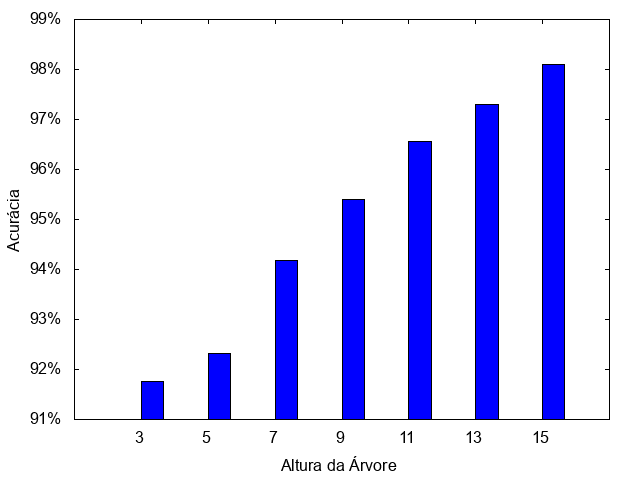
\includegraphics[scale=0.7]{tree-depth.png}
    \caption{Exemplo genérico de um gráfico ou figura que pode ser colocao aqui para representar os resultados quantitativos.}
    \label{fig:depth}
\end{figure}

\section{Conclusões}

Aqui o autor deve fazer uma reflexão sobre os achados da revisão sistemática. Esteja atento para acrescentar informação nova, ou seja, para "Concluir" de fato alguma coisa e não para repetir a análise da seção anterior. 

Devem ser inclusive apontadas as lacunas e limitações identificadas a partir da revisão sistemática, fazendo link com as possíveis propostas que serão apresentadas futuramente no anteprojeto. Ou seja, a conclusão deste relatório deve preparar o alicerce para a construção do anteprojeto de pesquisa. 



\bibliographystyle{sbc}
\bibliography{RT1}

\pagebreak
\begin{landscape}


\section{Planilha-resumo de Resultados}

Aqui deve ser atualizada a planilha-resumo contendo todos os trabalhos selecionados após a fase de seleção. A tabela deve conter todas as colunas indicadas a seguir com as informações relevantes sobre os trabalhos lidos na íntegra. Ver o exemplo na Tabela \ref{tab:resumo}.

\begin{center}
    
 
    \begin{longtable}{p{8cm}|c|c|c|c|c|p{7cm}|p{5cm}}
     \caption{Planilha-resumo dos trabalhos selecionados.}
    \label{tab:resumo} \\
     \multicolumn{1}{c|}{\textbf{Identificação do Trabalho}} &
     \multicolumn{1}{c|}{\textbf{I1}} &
     \multicolumn{1}{c|}{\textbf{I2}} &
     \multicolumn{1}{c|}{\textbf{I3}} &
     \multicolumn{1}{c|}{\textbf{E1}} &
     \multicolumn{1}{c|}{\textbf{E2}} &
     \multicolumn{1}{c|}{\textbf{Descrição}} & \multicolumn{1}{c}{\textbf{Avaliação}} \\ \hline \hline
    \endfirsthead

    \multicolumn{8}{c}%
    {{\bfseries \tablename\ \thetable{} -- continuação da página anterior}} \\
    \multicolumn{1}{c|}{\textbf{Identificação do Trabalho}} &
     \multicolumn{1}{c|}{\textbf{I1}} &
     \multicolumn{1}{c|}{\textbf{I2}} &
     \multicolumn{1}{c|}{\textbf{I3}} &
     \multicolumn{1}{c|}{\textbf{E1}} &
     \multicolumn{1}{c|}{\textbf{E2}} &
     \multicolumn{1}{c|}{\textbf{Descrição}} & \multicolumn{1}{c}{\textbf{Avaliação}} \\ \hline \hline 
    \endhead

    \hline \multicolumn{8}{r}{{Continua na próxima página}} \\ 
    \endfoot
    \hline \hline
    \endlastfoot
         
    
         \bibentry{Laranjeira2015} & X & & & & & Aqui é colocada a descrição do artigo com os dados resultantes da etapa de extração, após leitura completa do trabalho. & Aqui é feita avaliação do que foi encontrado neste artigo. Esta informação será útil para a avaliação qualitativa dos resultados. \\
         \hline
         \bibentry{breiman2017classification} & & & X & & X & Aqui é colocada a descrição do artigo com os dados resultantes da etapa de extração, após leitura completa do trabalho. & Aqui é feita avaliação do que foi encontrado neste artigo. Esta informação será útil para a avaliação qualitativa dos resultados. \\
         \hline
         \bibentry{SimoesEtAl2016-BRAHUR} & & X & X & & & Aqui é colocada a descrição do artigo com os dados resultantes da etapa de extração, após leitura completa do trabalho. & Aqui é feita avaliação do que foi encontrado neste artigo. Esta informação será útil para a avaliação qualitativa dos resultados. \\
         \hline
         
         
         
    \end{longtable}

    
\end{center}

\end{landscape}
\end{document}
